% fork-existence.tex

\documentclass{standalone}
% newcommands.tex

\newcommand{\enq}{\texttt{enq}}
\newcommand{\deq}{\texttt{deq}}
\newcommand{\pput}{\texttt{PUT}}
\newcommand{\get}{\texttt{GET}}
\newcommand{\vs}{\texttt{vis}}
\newcommand{\so}{\texttt{so}}
\newcommand{\arb}{\texttt{ar}}
\newcommand{\rf}{\texttt{rf}}

% example
\newcommand{\po}[2]{\draw [->, thick] (#1) to node[above] {\Large{\so}} (#2);}
\newcommand{\pva}[2]{\draw [->, thick] (#1) to node[above] {$\Large{\so},\Large{\vs},\Large{\arb}$} (#2);}
\newcommand{\pbva}[2]{\draw [->, thick] (#1) to node[above] {$\Large{\so}$} node[below] {$\Large{\vs},\Large{\arb}$} (#2);}
\newcommand{\pv}[2]{\draw [->, thick] (#1) to node[above] {\Large{\so}} node[below] {\Large{\vs}} (#2);}
\newcommand{\evis}[2]{\draw [->, thick] (#1) to node[above, sloped, near end] {\Large{\vs}} (#2);}
\newcommand{\mvis}[2]{\draw [->, thick] (#1) to node[above, sloped] {\Large{\vs}} (#2);}
\newcommand{\ar}[2]{\draw [->, thick, allow upside down] (#1) to node[above, sloped] {\Large{\arb}} (#2);}
\newcommand{\va}[2]{\draw [->, thick, allow upside down] (#1) to node[above, sloped] {$\Large{\vs},\Large{\arb}$} (#2);}
\newcommand{\vab}[2]{\draw [->, thick, allow upside down] (#1) to node[below, sloped, near end] {$\Large{\vs},\Large{\arb}$} (#2);}
\newcommand{\vae}[2]{\draw [->, thick, allow upside down] (#1) to node[above, sloped, near end] {$\Large{\vs},\Large{\arb}$} (#2);}
\newcommand{\vas}[2]{\draw [->, thick, allow upside down] (#1) to node[sloped, near start, above] {$\Large{\vs},\Large{\arb}$} (#2);}

% serialization
\newcommand{\scc}[2]{\draw [->, very thick] (#1) to (#2);}
\newcommand{\rva}[2]{\draw [->, thick, allow upside down] (#1) to node[above, sloped] {$\Large{\rf},\Large{\vs},\Large{\arb}$} (#2);}
\newcommand{\rvb}[2]{\draw [->, thick, allow upside down] (#1) to node[below, sloped] {$\Large{\rf},\Large{\vs},\Large{\arb}$} (#2);}


\usepackage{tikz}
\usetikzlibrary{shapes, positioning, arrows.meta, decorations.pathmorphing}

\begin{document}
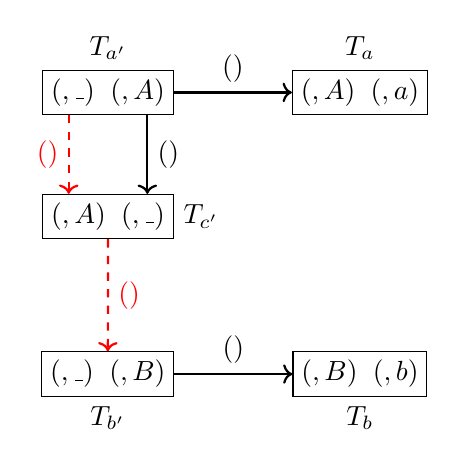
\begin{tikzpicture}[
  node distance = 3.0cm and 1.5cm,
  wr/.style = {->, thick},
  ww/.style = {->, thick, dashed, red},
  rw/.style = {->, thick, dotted, blue},
  txn/.style = {draw, inner sep = 3pt, align = center}]

  \node[txn, label = above : $T_{a}$] (ta)
    {$\readevent(\keyxvar, A)\;\;\writeevent(\keyxvar, a)$};
  \node[txn, label = below : $T_{b}$, below = of ta] (tb)
    {$\readevent(\keyxvar, B)\;\;\writeevent(\keyxvar, b)$};

  \node[txn, label = above : $T_{a'}$, left = of ta] (ta-prime)
    {$\readevent(\keyxvar, \_)\;\;\writeevent(\keyxvar, A)$};
  \node[txn, label = below : $T_{b'}$, left = of tb] (tb-prime)
    {$\readevent(\keyxvar, \_)\;\;\writeevent(\keyxvar, B)$};

  \node[txn, label = right : $T_{c'}$, below = 1.0cm of ta-prime] (tc-prime)
    {$\readevent(\keyxvar, A)\;\;\writeevent(\keyxvar, \_)$};

  \draw[wr, sloped] (ta-prime) to node[above]{$\WR(\keyxvar)$} (ta);
  \draw[wr, sloped] (tb-prime) to node[above]{$\WR(\keyxvar)$} (tb);

  \draw[wr] (ta-prime.-30) to node[right]{$\WR(\keyxvar)$} (ta-prime.-30 |- tc-prime.north);
  \draw[ww] (ta-prime.-150) to node[left]{$\WW(\keyxvar)$} (ta-prime.-150 |- tc-prime.north);
  \draw[ww] (tc-prime) to node[right]{$\WW(\keyxvar)$} (tb-prime);
\end{tikzpicture}
\end{document}